
\documentclass[10pt,english]{article}
\usepackage[bottom=0.8in,margin=0.8in]{geometry}
\geometry{a4paper}
\usepackage[english]{babel}
\usepackage{indentfirst}
\selectlanguage{english}
\usepackage{multicol}
%\usepackage{varioref}% smart page, figure, table, and equation referencing
\usepackage[colorlinks]{hyperref}% hyperlinks [must be loaded after dropping]
\hypersetup{colorlinks,breaklinks,
citecolor = blue,
urlcolor=blue,
linkcolor=blue}
\usepackage[noabbrev]{cleveref}

\usepackage{placeins}
\usepackage[utf8]{inputenc}



\usepackage{graphicx}

\usepackage{amssymb}
\usepackage{authblk}
\graphicspath{{../Proj_Output/}} % allows figures to be placed in a different folder



\title{\vspace{-20pt}CFD Convergence Studies on a Deformable Membrane in a Channel}
\author{Kevin R. Moore}
\affil{\vspace{-10pt}Brigham Young University}
\renewcommand\Authands{, }
\date{}

\begin{document}

\maketitle
\vspace{0pt}
%\section{Project Overview}
   \textbf{As part of the BYU Computational Fluids and Heat Transfer graduate level course, we are to achieve a familiarity with various commercial software while learning the proper numerical and theoretical techniques.  The four specific objectives in this study were to: First, recreate the geometry and flow conditions of the coupled fluid-solid interface between a flexible membrane in a fluid filled channel as detailed in \textit{A Numerical Simulation of Steady Flow in a 2-D Collapsible Channel} by Luo and Pedley. Second, perform a grid independence study.  Third, demonstrate convergence criteria independence for the solid, fluid, and coupled FSI convergence criteria.  Fourth, exercise the model by recreating a sweep of beam tension factor.  }

\vspace{0pt}

\section{Model Overview}

Following the descriptions by Luo and Pedley, I reconstructed the flexible channel and beam as seen in \cref{f:setup}.  Further, in order to facilitate better meshing, and a leader-follower relationship during the large deformations, I broke the flexible beam section into five evenly spaced segments.  The specific fluid and geometric parameters can be found in \cref{tab:params}.  The beam had an external pressure applied as well as a pretension.    All modeling was done using first order elements in the Adina programming language and interface.

\begin{figure}[htbp]
\centering
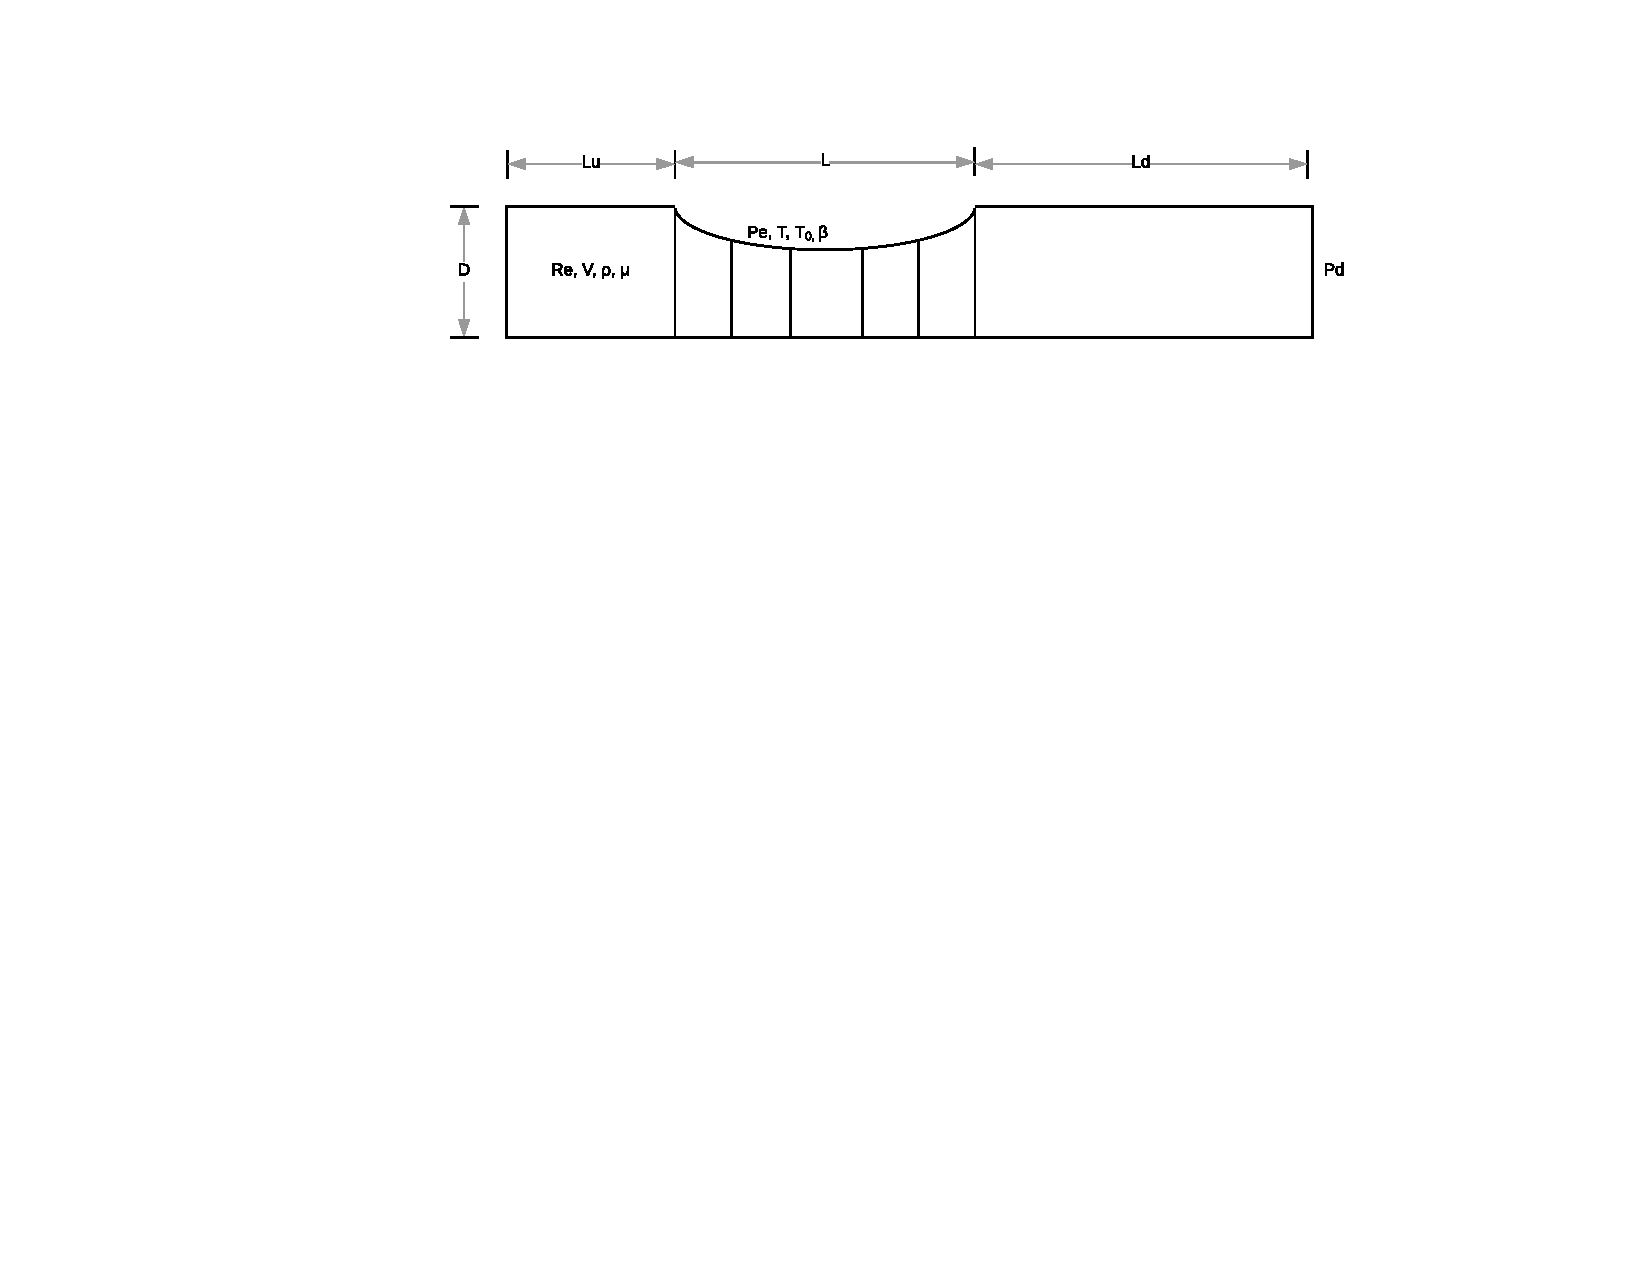
\includegraphics[trim={7.5cm 15.5cm 5.6cm 2.5cm},clip,width=0.95\textwidth]{Adina_Setup}
\caption{Illustration of the experimental setup and sectioning for meshing, not to scale.}
\label{f:setup}
\end{figure}

\begin{table*}[h]
\vspace{20pt}
\centering
  \begin{tabular}{lcl}
    \textbf{Name} & \textbf{Value} & \textbf{Description}  \\
    Lu & 2E-2 m & Upper channel length  \\
    L & 5E-2 m & Flexible member length\\
    Ld & 7E-2 m & Downward channel length\\
    D & 1E-2 m & Channel height\\
    $\rho$  & 1E3 m/kg & Fluid density\\
    $\mu$  & 1E3 Pa-s & Fluid viscosity\\ 
   $T$  & 1E3-0 Pa & Beam pre-tension \\
    $T_0$  & 1E3 Pa & Beam baseline tension \\ 
   Pe  & 0.93 Pa & Beam external pressure \\ 
  E  & 1 Pa & Beam stiffness \\ 
   Re  & 100-500 & Average inlet velocity Reynolds number\\ 
  V  & $\frac{Re \mu 3}{\rho D 2}$ & Inlet centerline velocity \\ 
  $\bar{U}$  & $\frac{Re \mu}{\rho D}$ & Mean inlet velocity \\ 
    h  & 1E-4 m & Beam thickness \\ 
    $\beta$  & $\frac{T_0}{T}$ & Beam tension factor \\ 
  \end{tabular}
  \caption{Summary of channel geometry and fluid/structure variables.}
  \label{tab:params}
\end{table*}

\newpage

To make better use of mesh elements, I created a progressive refinement with respect to the lengthwise direction of the channel.  As seen in \cref{f:grid_1_5}, the mesh coarsens at the inlet and outlet where lengthwise gradients should be small.  Though not seen in the figure, the beam elements match the discretization of the fluid domain.

\begin{figure}[htbp]
\centering
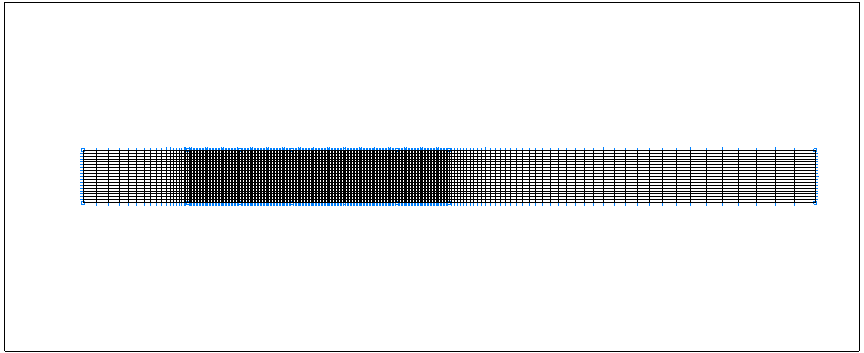
\includegraphics[trim={2.85cm 5cm 1.6cm 4cm},clip,width=0.98\textwidth]{Mesh1_5.png}
\caption{Example mesh grid showing progressive refinement around the flexible beam area.}
\label{f:grid_1_5}
\end{figure}

The coupled fluid-solid simulation was modeled in the time domain with Rayleigh Damping to enable better numerical convergence.  Alpha was set to 70 and beta was set to 1.  Additionally, the pressure on the beam and the fluid inlet velocity was ramped up over a coarse time step to further increase numerical damping and successful convergence.  The time step was 1 second, the FSI (fluid solid interface) was set to iterate for 100 times per time step, total time steps was 70, and the linear ramp for both the fluid velocity and beam pressure was at full value at 40 time steps.   


\vspace{5pt}
\section{Grid Independence}

To verify grid independence, the mesh domain was parameterized to allow for an arbitrary number of elements divisible by five and was run with successively doubled number of mesh elements.  The fluid and solid parameters were set to: Re = 500 and $\beta$ = 16.5.   \Cref{f:3b} shows the vorticity distribution across the upper surface of the beam for each of the element numbers.  Deviating from Luo and Pedley, I needed an order of magnitude more elements in order resolve the FSI simulation fully with my grid independent solution being the 30k element case while theirs was around a tenth of that.  Node numbers followed the number of elements closely (ex. the 30240 element case had 31,117 nodes) due to the first order nature of the 4 node elements used.

\begin{figure}[htbp]
\centering
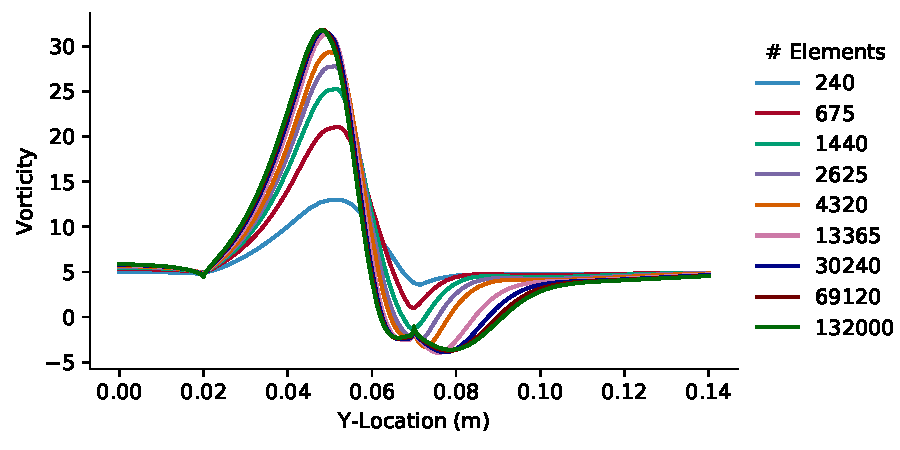
\includegraphics[trim={.0cm .25cm .0cm 0cm},clip,width=0.75\textwidth]{fig3b}
\vspace{-5pt}
\caption{Distribution of vorticity across the upper channel surface.  Vorticity is nondimensionalized by $\omega$ = $\frac{\omega D}{\bar{U}}$.  Using first order elements makes node numbers slightly larger than elements due to outer nodes. Re = 500 and $\beta$ = 16.5}
\label{f:3b}
\end{figure}

To make the convergence criteria clearer, I plotted the maximum vorticity as a function of element number as seen in \cref{f:3b_max}.  It should be noted that for the 8k element case, I made a mistake in properly capturing the output data by mis-selecting the output variable.  That case was set to 0 for plotting purposes.

\Cref{f:3b_time_cells} shows the time to solve, which is linear as expected for the first order element type.  It is possible that I may have been able to cut the simulation time down by increasing the speed of the ramp and decreasing the number of time steps.  However, I was satisfied with the required time to solved for this 2D case.  \\

\vspace{10pt}
\begin{figure}[h]
\centering
\begin{minipage}{.58\textwidth}
  \centering
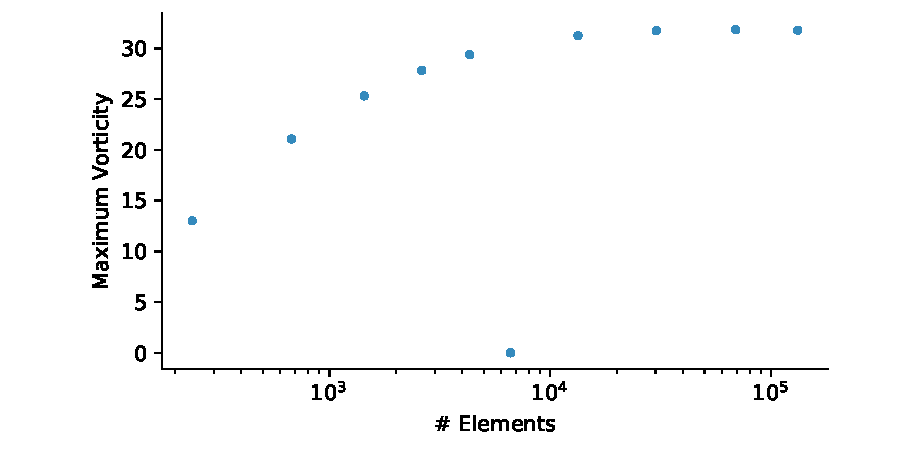
\includegraphics[trim={1.2cm 0cm .0cm 0cm},clip,width=0.98\textwidth]{fig3b_max}
  \caption{Maximum vorticity of \cref{f:3b} plotted against element number, grid converged at approximately 30k elements.  The 8k case data was incorrect due to human error in data extraction.}
\label{f:3b_max}
\end{minipage}%
\hspace{5pt}
\begin{minipage}{.38\textwidth}
  \centering
  \vspace{20pt}
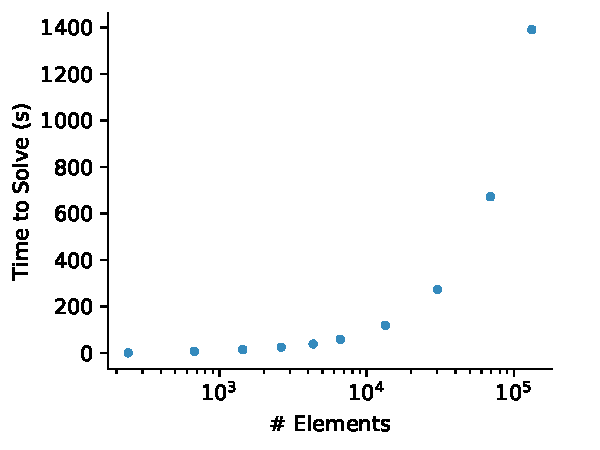
\includegraphics[trim={.1cm 0cm .5cm .2cm},clip,width=0.98\textwidth]{fig3b_time_cells}
\vspace{-8pt}
  \caption{Time to solve increases linearly with number of elements as is expected for the first order element type. }
\label{f:3b_time_cells}
\end{minipage}
\end{figure}

\newpage
Figures \ref{f:Mesh0_5_Contour} and \ref{f:Mesh5_0_Contour} show the vorticity band plots over the entire fluid domain.  I apologize for the rainbow color scheme.  Both band plots have corresponding colors ranging from -100 to 100.  It can clearly be seen that the coarse mesh solution does not deform as much as the fine mesh, which in turn decreases the fluid velocity in the narrowest part of the channel and in turn vorticity.  

\vspace{30pt}

\begin{figure}[h!]
\centering
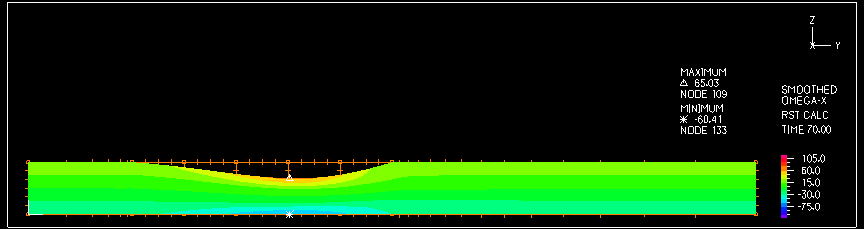
\includegraphics[trim={0.8cm 0.2cm 0.7cm 0.2cm},clip,width=0.98\textwidth]{Mesh0_5_Contour.png}
\caption{Coarse 240 element grid mesh vorticity contour plot differs notably from the fine solution in \cref{f:Mesh5_0_Contour}.  Color legends are consistent.}
\label{f:Mesh0_5_Contour}
\end{figure}

\vspace{20pt}

\begin{figure}[h!]
\centering
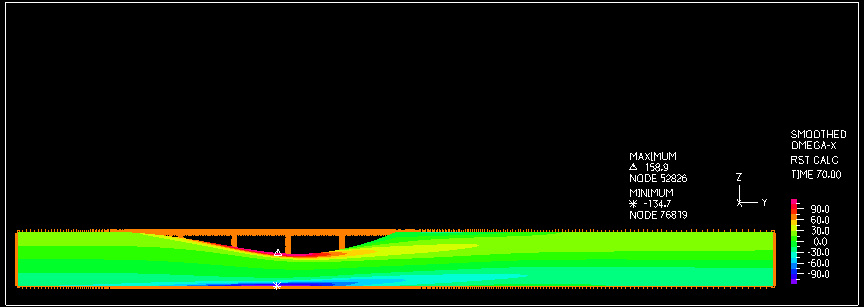
\includegraphics[trim={0.5cm 0.2cm 0.6cm 3.5cm},clip,width=0.98\textwidth]{Mesh5_0_Contour.png}
\caption{Fine 132,000 element grid mesh vorticity contour plot.}
\label{f:Mesh5_0_Contour}
\end{figure}


\newpage
\section{Convergence Criteria Independence}

To verify convergence criteria independence, specifically fluid degrees of freedom tolerance, solid energy tolerance, and FSI force and displacement, all three criteria were set to the same value and iteratively changed by an order of magnitude.  The same simulation parameters as before were used.  The 30k element case from the grid convergence was used for these simulations.  \Cref{f:3bTOL} shows that the effect on the vorticity is minor: arguably negligent.  


\begin{figure}[h!]
\centering
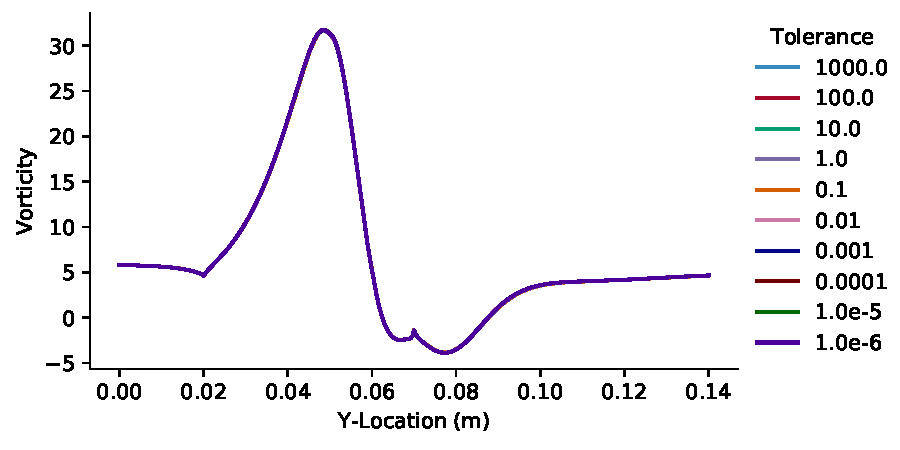
\includegraphics[trim={.0cm .25cm .0cm 0cm},clip,width=0.70\textwidth]{fig3b_TOL}
\vspace{-10pt}
\caption{Vorticity as a function of solver tolerance shows little variance.}
\label{f:3bTOL}
\end{figure}

To get a better visual on the change in vorticity as a function of solver tolerance I plotted the maximum vorticity as a function of tolerance, see \cref{f:3bTOL_max}.  The solution appears to be solver tolerance independent below 1E-4 and a cap with a maximum of 1.0.  Regarding the time to solve as seen in \cref{f:3bTOL_time_cells}, the additional computational expense appears to increase in a base 10 manner.\vspace{40pt}
\begin{figure}[h!]
\centering
\begin{minipage}{.49\textwidth}
  \centering
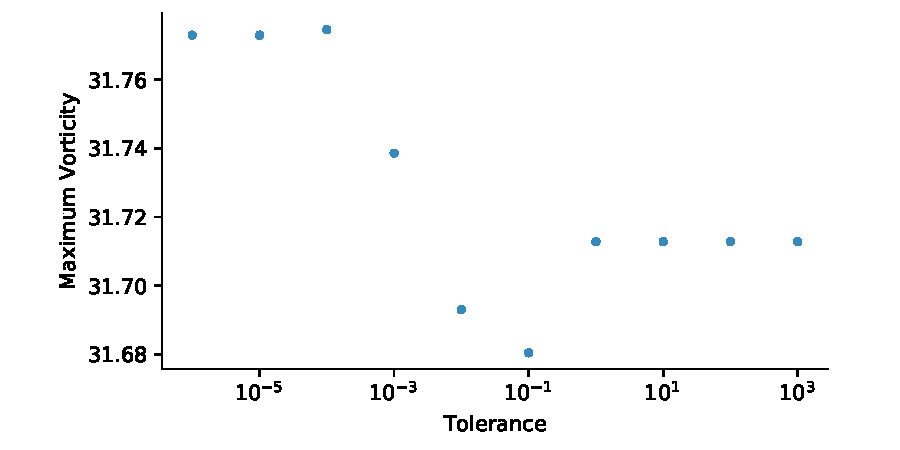
\includegraphics[trim={1.0cm 0cm 1.4cm 0cm},clip,width=0.98\textwidth]{fig3b_TOL_max}
\vspace{3pt}
\caption{Maximum vorticity shows a solver tolerance independent solution past 1E-4.}
\label{f:3bTOL_max}
\end{minipage}%
\hspace{5pt}
\begin{minipage}{.49\textwidth}
  \centering
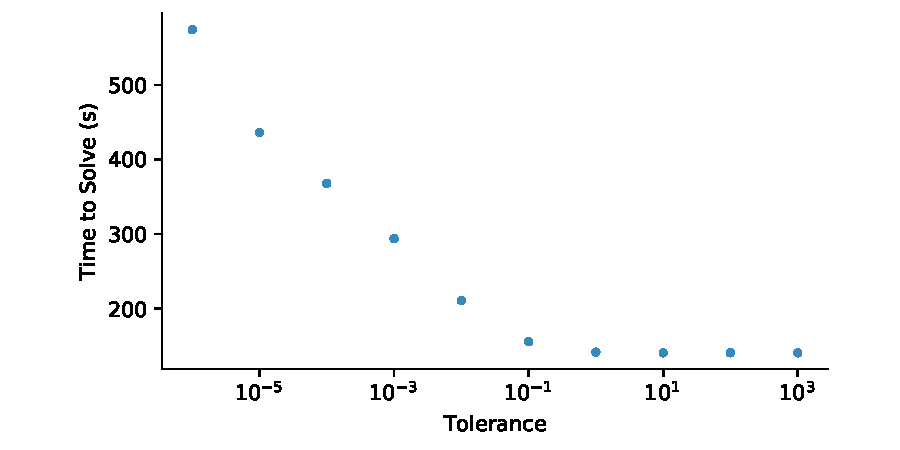
\includegraphics[trim={1.0cm 0cm 1.4cm .5cm},clip,width=0.98\textwidth]{fig3b_TOL_time_cells}
\caption{Time to solve increases in a base 10 manner.}
\label{f:3bTOL_time_cells}
\end{minipage}
\end{figure}

\section{Model Exersize}
Using the grid and solver independent simulation parameters for the element count and convergence criteria, I exercised the model by recreating figure 5 from Luo and Pedley.  For this simulation, Re was set to 100 and $\beta$ was varied from 1 to 150.  Three outputs were measured: beam deflection, pressure along the top surface, and vorticity along the top surface.  The non-dimensionalization of the vorticity has been previously defined in \cref{f:3b}, and the scaling of the pressure is defined in Luo and Pedley's paper.  For each of the cases, I hand picked the data from the plots given in the original article and as such, the values are only representative of the original study and not precise recreations.  The following three figures (\ref{f:fig5_def}, \ref{f:fig5_press}, and \ref{f:fig5_vor} follow the same order and general format as figure 5 from Luo and Pedley including the original data and results from this study.  In all three cases, only minor variances in the solution were observed.



\begin{figure}[h!]
\centering
\vspace{-0pt}
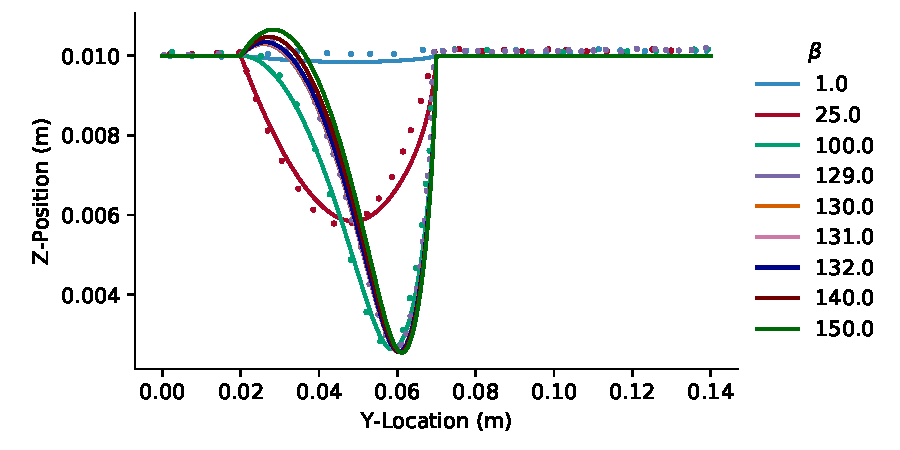
\includegraphics[trim={.0cm 0cm .0cm 0cm},clip,width=0.85\textwidth]{fig5_def}
\caption{Beam deformation shows good agreement with original study. For $\beta$ = 25.0 shows a slightly skewed curve.  Solid lines: current study.  Dots: Luo and Pedley data acquired by hand. }
\label{f:fig5_def}

\centering
\vspace{-0pt}
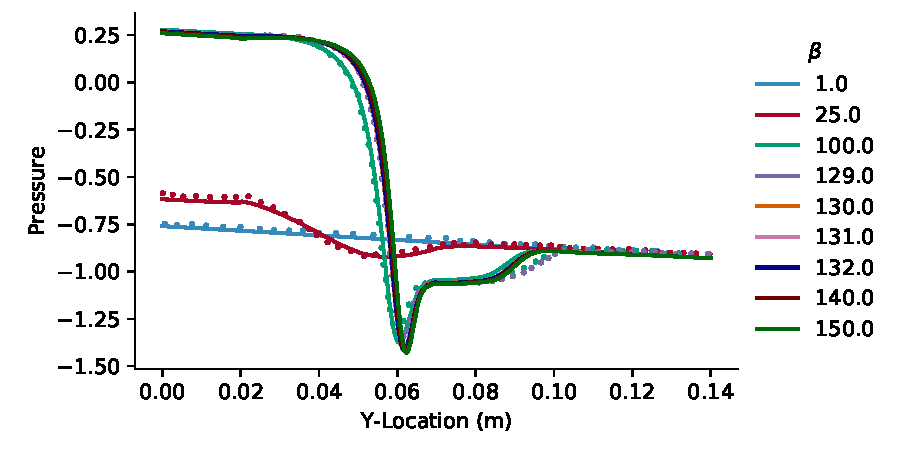
\includegraphics[trim={.0cm 0cm .0cm 0cm},clip,width=0.85\textwidth]{fig5_press}
\caption{Pressure distrubution shows good agreement with original study.  Between Y = 0.09-0.1 shows some deviation.  Solid lines: current study.  Dots: Luo and Pedley data acquired by hand.}
\label{f:fig5_press}

\centering
\vspace{-0pt}
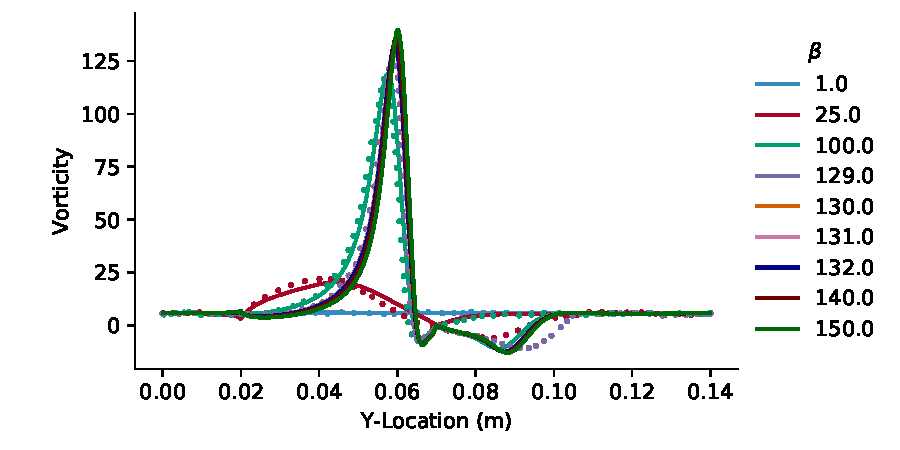
\includegraphics[trim={.0cm 0cm .0cm 0cm},clip,width=0.85\textwidth]{fig5_vor}
\caption{Vorticity distribution shows similar agreement with pressure distribution including error in the Y = 0.09-0.10 region. Solid lines: current study.  Dots: Luo and Pedley data acquired by hand.  It should be noted that for the $\beta$ = 25.0 case, the hand picked data follows the wrong curve after Y = 0.07.}
\label{f:fig5_vor}
\end{figure}


\FloatBarrier
As can be seen in the plots above, no spurious pressure fluctuations were observed.  Seeing the results from Luo and Pedley, I was under the impression that the pressure would diverge at around the same $\beta$ value, however this did not happen.  In fact, it appears that $\beta$ has a relatively small effect on the solutions after a value of 140.  It is possible that the model I created has significantly larger damping characteristics due to the very coarse time step and included Rayleigh Damping.  I ran the model up to $\beta$ = 150.0 without problems and have heard of peers successfully running up to a value of 250.0.  Vorticity and pressure contour plots can be seen in figures \ref{f:CFD_B150_vorticity_band} and \ref{f:CFD_B150_pressure_band}.\\

\begin{figure}[h!]
\centering
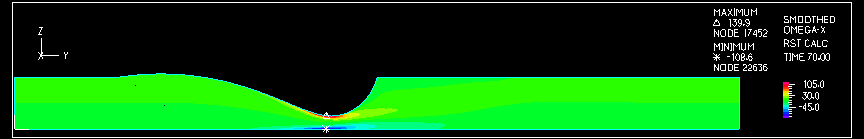
\includegraphics[trim={0.4cm 0.2cm 0.7cm 0.2cm},clip,width=0.98\textwidth]{CFD_B150_vorticity_band.png}
\caption{$\beta$ = 150 vorticity contour plot.}
\label{f:CFD_B150_vorticity_band}
\end{figure}

\vspace{0pt}

\begin{figure}[h!]
\centering
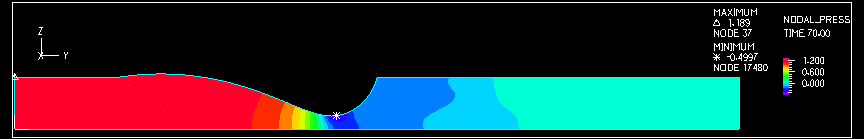
\includegraphics[trim={0.4cm 0.2cm 0.4cm 0.2cm},clip,width=0.98\textwidth]{CFD_B150_pressure_band.png}
\caption{$\beta$ = 150 pressure contour plot.}
\label{f:CFD_B150_pressure_band}
\end{figure}

\section{Conclusions}

Overall, the results from the Adina FSI simulation matched closely with those found by Luo and Pedley and the objectives for this project were met: I demonstrated grid and solver criteria independence, gained experience with a foreign CFD/FEA solver software, and had the opportunity to practice recreating results from previous researchers.  The experience gained during this project will be a great benefit to me as I continue striving to produce high quality and impactful research in fluids related areas of interest.

Challenges faced were primarily related to digging up the required parameters and assumptions in the original paper in order to create a similar solution.  The secondary challenge I encountered was the availability of the Adina software: even though I had access to it via CAEDM Labs and RGS clients, I continuously ran into non-Adina problems.  I estimate 40 hours of work was required for this project.  If a way to run an Adina .in script including post processing via the terminal was provided, I may have been able to cut out about 5 hours of repetitive button clicking and typing for the post processing and plotting steps.

\end{document}
